
%(BEGIN_QUESTION)
% Copyright 2011, Tony R. Kuphaldt, released under the Creative Commons Attribution License (v 1.0)
% This means you may do almost anything with this work of mine, so long as you give me proper credit

Calculate the necessary weight applied to the piston of this deadweight tester to produce a pressure of 300 PSI, assuming a primary piston diameter of 0.136 inches and a secondary piston diameter of 0.25 inches.  Also, calculate the necessary force applied by the secondary piston on the oil to produce this pressure:

\vskip 10pt

$$\includegraphics[width=15.5cm]{i03572x01.eps}$$

\vskip 10pt

Required weight = \underbar{\hskip 50pt} pounds

\vskip 10pt

Required secondary piston force = \underbar{\hskip 50pt} pounds 

\underbar{file i03572}
%(END_QUESTION)





%(BEGIN_ANSWER)

\noindent
5 points for each answer:

\vskip 10pt

Required weight = \underbar{\bf 4.358} pounds

\vskip 10pt

Required secondary piston force = \underbar{\bf 14.73} pounds 

%(END_ANSWER)





%(BEGIN_NOTES)

{\bf This question is intended for exams only and not worksheets!}.

%(END_NOTES)


